\section{The \ModelName}
\label{sec:model}
% Sanders~\cite{sanders2009security} argues that existing security metrics should be integrated to provide a comprehensive, quantified view of systems through their lifecycle. 
To make claims about how security practices affect security outcomes, we need to account for other influences on security outcomes. We propose the \ModelAbbr model of the factors influencing security outcomes in software development to enable assessment of how varying security practice use affects those outcomes, while accounting for software usage's effect. 
 
 The Common Criteria (CC) introduction~\cite{common2012common} lists a set of \textbf{security concepts} (concepts bolded) and relationships, summarized as follows:
 \begin{itemize}
 	\item  Owners value \textbf{Assets} and  impose \textbf{Countermeasures} to reduce \textbf{Risk}.
 	\item Threat Agents give rise to \textbf{Threats} that affect \textbf{Assets} and increase \textbf{Risk}.
 \end{itemize}
 
 Considering the CC concepts in the context of software development and use, we propose a model to capture the distinction between the risk to Assets caused by Threats (Usage Risk) and the risk caused by the software that manages the Assets (Development Risk)  when measuring practice Adherence's effect on security Outcomes.  

We have theorized relationships between measurement variables and each construct in our model. For example, we theorize that the already mentioned code size and code churn metrics influence Development Risk. We present our list of measurements in Section \ref{sec:model_measurement}, and present the construct relationships in the `Construct' column for each metric in Table~\ref{tab:model_spef_metrics}.

\subsection{Structural Model Constructs}
 \label{sec:model_structual}
In this section, we define the Development Risk, Usage Risk, Adherence, and Outcomes constructs, and the relationships we expect between each construct. 

\subsubsection{Development Risk}
Development Risk (CC \textbf{Risk} potential) represents the characteristics of the software produced by the development team that are associated with defects and vulnerabilities. In the case of software vulnerabilities, for example, high code churn~\cite{shin2011evaluating} and defect-prone languages~\cite{ray2014a} are two examples of software attributes that have been correlated with vulnerabilities. See Catal and Diri~\cite{catal2009a}, and Morrison et al.~\cite{morrison2014mapping} for two examples of surveys of vulnerabilty-related metrics. 

\subsubsection{Usage Risk}
Usage Risk (CC \textbf{Assets}) represents the characteristics of the software's purpose and usage context that are associated with attacker interest. One component of attacker interest is the value of the assets managed by the software. For example, we conjecture that software tracking valuable or sensitive data, such as Personally Identifiable Information (PII) or credit card data is more likely to be attacked than software tracking, say, baseball scores. As another example, attacker control over a machine enables the machine's participation in a botnet, making the number of machines on which a piece of software runs a consideration in evaluating the software's Usage Risk.

\subsubsection{Adherence}
\label{sec:model_contruct_adherence}
Adherence (CC \textbf{Countermeasures}) represents the efforts the team takes to prevent and discover vulnerabilities. When effort is reported for security practice evaluations in the software engineering literature, it is typically reported in terms of time spent. For example, Austin et al.~\cite{austin2011one} measured the time required to apply penetration testing tools, static analysis tools, and testing to locate vulnerabilities, and Dowd et al.~\cite{dowd2006the} reports security code review rates of 100-1000 SLOC per hour. 

In the information technology literature, 
researchers have developed `technology adoption' models for how technology users adhere to new technologies. Davis' ~\cite{davis1986tam} Technology Acceptance Model (TAM) posits perceived usefulness and perceived ease of use as constructs central to a user's intention to use a given technology, and TAM has been applied and reviewed extensively, e.g. Venkatesh ~\cite{venkatesh2003user}. Venkatesh ~\cite{venkatesh2003user} examined TAM and seven related models and extensions to TAM, and proposed the Unified Theory of Acceptance and Use of Technology (UTAUT) model. UTAUT retains the TAM constructs, while adding Social Influence and Facilitating Conditions as primary constructs driving user intention to use a given technology. 

% emails - spec
% commit messages - code
% tests - test
% issues - ops
% documentation - spec

\subsubsection{Outcomes}
\label{sec:model_contruct_outcome}
The Outcomes (CC \textbf{Risk} realized) construct represents indications of the failure or achievement of security associated with a piece of software over the course of the software's life cycle.

 At present, counting vulnerabilities is the most common means of measuring security in software~\cite{morrison2014mapping}. However, as pointed out by Meneely~\cite{meneely2016security}, vulnerabilities measure breaches in security rather than the presence of security. Where possible, analogues to the reliability engineering measurement of mean time between failure should be measured for the assessment software security. 

\subsection{Structural Model Relationships}
We hypothesize that the four constructs are related as follows:
\begin{itemize}
	\item \textbf{H1} Usage Risk is associated with negative Security Outcomes
	\item \textbf{H2} Development Risk is associated with negative Security Outcomes
	\item \textbf{H3} Development Risk is inversely associated with Practice Adherence  	
\end{itemize}

For example, a carefully designed, written, and tested piece of widely-used software that manages financial data (high Usage Risk, low Development Risk, e.g. Bitcoin with 22 CVEs~\footnote{\url{https://www.cvedetails.com/vulnerability-list/vendor_id-12094/Bitcoin.html}}) might have poorer Outcomes than a less well written baseball scores program used by a few hundred users (low Usage Risk, high Development Risk, no CVEs reported) because attackers expend more effort on the software managing financial data. We would expect Adherence to be correlated with Usage Risk, as teams adopted security practices in proportion to the security needs of their software, its usage context, and their users. In practice, for example in the case of the CloudBleed example from the introduction of this paper, users (especially attackers) sometimes surprise development teams in the uses of their software, unexpectedly increasing the software's Usage Risk out of proportion to the team's Adherence. 

Figure~\ref{fig:model_constructs} depicts the constructs and their relationships.  Each circle in the figure represents a construct, modeled as a `latent variable'. We model the constructs using latent variables to indicate that our measures for each construct are aggregates of the measurement (observed) variables ~\cite{kline2015principles,borsboom2008latent}. 

 \begin{figure}
 	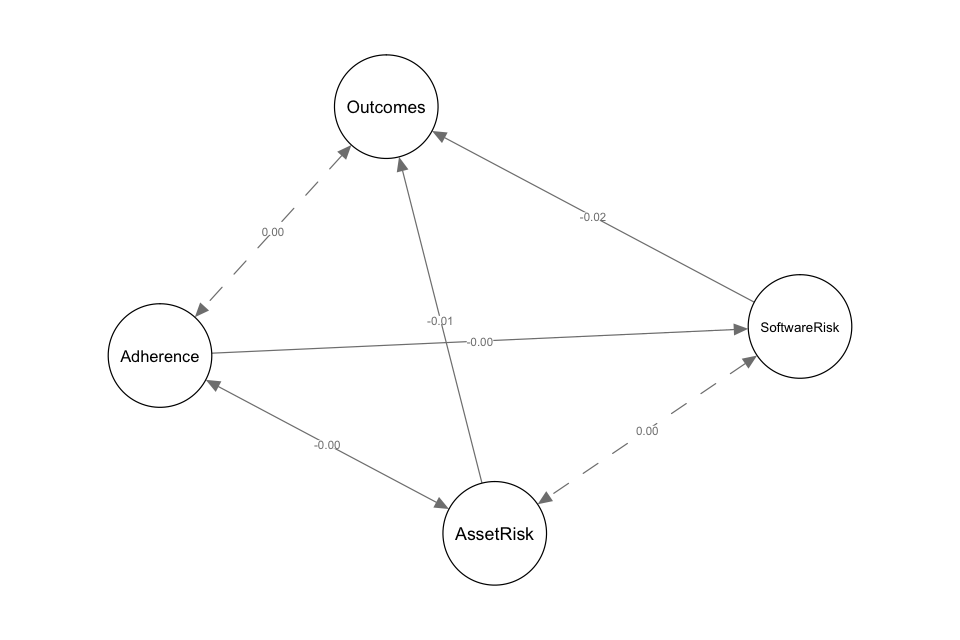
\includegraphics[width=\columnwidth]{modelzeroB.png}
 	\caption{Structural Model Overview}
 	\label{fig:model_constructs}
 \end{figure}
 
Directed edges from circles to other circles, for example the arrow from Usage Risk to Outcomes in Figure \ref{fig:model_constructs}, represent a source latent variable's effect on the target latent variable. SEM estimation generates parameter estimates for each edge. The sign and magnitude of the parameter estimate on the edge between variables represent how changes in a source variable covary (or correlate, for standardized estimates) with changes in a target variable in the direction of the parameter estimate's sign and of a magnitude comparable to other parameter estimates

Dual arrows between circles/constructs, for example between Adherence and UsageRisk in Figure \ref{fig:model_constructs}, represent covariances between the constructs, implying that a relationship exists, but that the direction of influence is not specified. Dual arrows starting and ending at the same variable indicate the variable's observed variance. 

Each square in Figure \ref{fig:model_example_syntax_asmeasuredby} represents a measurement variable associated with each construct. Directed edges (single arrows) from circles to squares, for example from DevelopmentRisk to SLOC as shown in Figure \ref{fig:model_example_syntax_asmeasuredby}, represent that a construct `is measured by' a measurement variable relationship. That is to say that the effect of the construct can be measured by the measurement variable. The parameter estimate on these relationships represents the sign and magnitude of the relative contribution of the measurement variable to the construct value. We present the list of measurements, and instructions for collecting them, for each construct in the SP-EF measurement guidebook~\cite{morrison2016spefguide}.

\begin{figure*}
	\centering
%	\begin{subfigure}{.5\textwidth}
		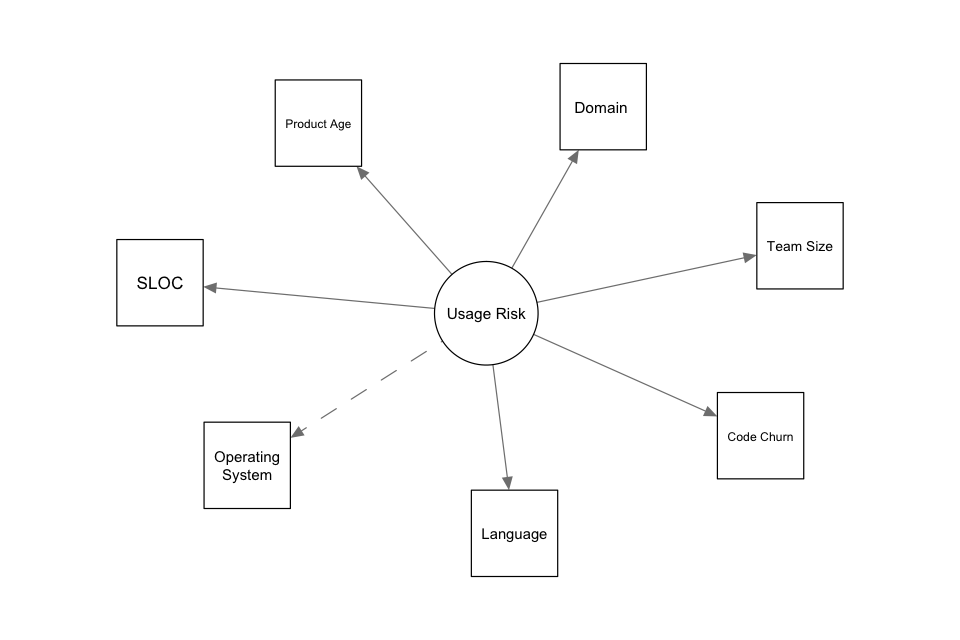
\includegraphics[width=1\textwidth]{syntax_usagerisk_asmeasuredby.png}
		\caption{Graphical display of lavaan syntax for DevelopmentRisk $=\sim$ Theorized measurement variables from Table  \ref{tab:model_spef_metrics}}
		\label{fig:model_example_syntax_asmeasuredby}	
%	\end{subfigure}%
%	\begin{subfigure}{.5\textwidth}		
%		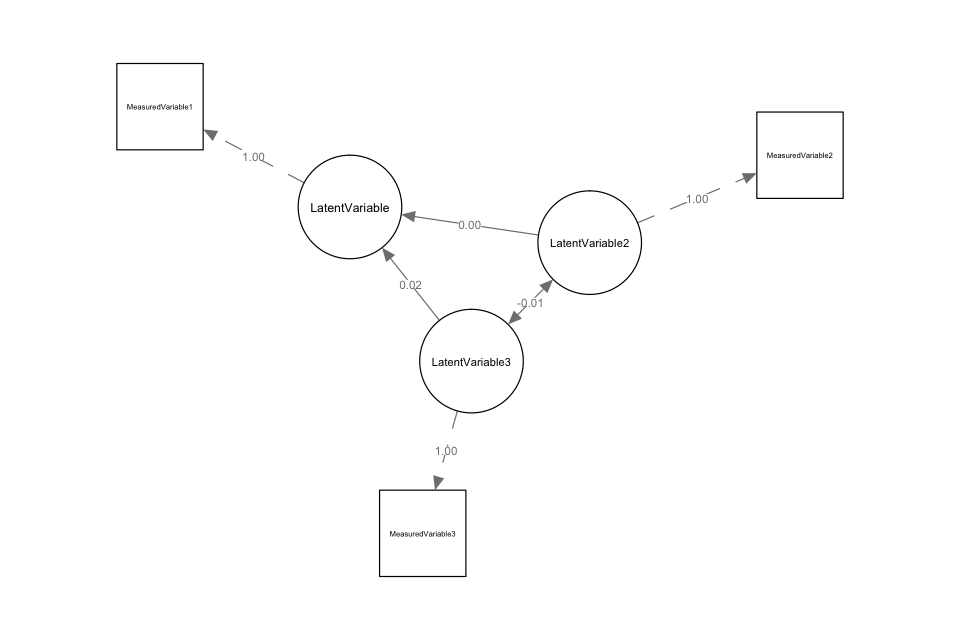
\includegraphics[width=.5\columnwidth]{syntax_latentregress.png}
%		\caption{Graphical display of lavaan syntax for $LatentVariable \sim LatentVariable2 + LatentVariable3$ (with measured variables)}
%		\label{fig:model_example_syntax_latentregress}	
%	\end{subfigure}		
\end{figure*}

%\begin{figure}
% \includegraphics[width=\columnwidth]{modelcaoscto}
%	\caption{Model Constructs and Sub-Constructs}
%	\label{fig:model_constructs_phases}
%\end{figure}


\subsection{Measurement Model: Metrics, Variables, and Relationships}
\label{sec:model_measurement}
%~\cite{morrison2014mapping}
%~\cite{morrison2016spefsite}
Through literature review~\cite{morrison2014mapping} and analysis~\cite{morrison2017surveying,morrison2017measuring}, we have developed a set of measurements that we expect to capture security-related constructs for software development. In Table \ref{tab:model_spef_metrics}, we name each data element, give our hypothesis about its relationship to the structural model construct, and cite a rationale for the data element's presence. The metrics associated with Development Risk and Usage Risk are termed Context Factors. The metrics associated with Adherence and Outcomes are termed Measures. 
		
\begin{table*}[!htbp] \centering 
	\caption{Model Context Factors, Measures, and Hypotheses} 
	\label{tab:model_spef_metrics} 
	\begin{scriptsize}
		\begin{tabular}{p{1.75cm}p{1cm}p{1cm}p{6cm}} 
			\\[-1.8ex]\hline 
		\hline \\[-1.8ex] 
		Metric & \multicolumn{1}{c}{Effect} & \multicolumn{1}{c}{Construct} & \multicolumn{1}{c}{Rationale} \\ 
		\hline \\[-1.8ex]  
			Language	& influences &	Development Risk &   Ray et al. ~\cite{ray2014a} and Walden et al. ~\cite{walden2010idea} found small but significant effects of programming language on software quality. Zhang~\cite{zhang2014towards} identifies language as a key context factor. \\
			Operating System	& influences &	Development Risk & \\	
			Domain &	influences &	Development Risk	 & Different risks are associated with different software domains~\cite{williams2004xpef,jones2000software} \\
			Product Age	& increases &	Development Risk & Kaminsky et al.~\cite{kaminsky2011showing} and Morrison et al.~\cite{morrison2015challenges} have found evidence of code age effects on the presence of vulnerabilities. \\
			Source Lines of Code (SLOC)	& influences	& Development Risk & Source code size is correlated with vulnerabilities ~\cite{shin2011evaluating}, ~\cite{alhazmi2007measuring}, ~\cite{camilo2015do} , ~\cite{dashevskyi2016on}. Zhang~\cite{zhang2014towards} identifies SLOC as a key context factor. \\
			Churn &	increases &	Development Risk  &  Code churn is correlated with vulnerabilities ~\cite{shin2011evaluating}.\\
			Team Size	& influences	& Development Risk & Shin et al. ~\cite{shin2011evaluating} and Zimmermann et al. ~\cite{zimmerman2010searching} found correlations between team size and vulnerabilities. \\			
			\hline \\[-1.8ex] 
			Number of Machines &	increases &	Usage Risk & (Proposed) The market for machine time on botnets suggests that the number of machines a piece of software runs on increases the software's desirability to attackers. \\
			Number of Identities &	increases &	Usage Risk	 &  (Proposed) The market for personal identities and credit card information suggests that the number of identities a piece of software manages increases the software's desirability to attackers.\\
			Number of Dollars &	increases &	Usage Risk & (Proposed) The amount of financial resources a piece of software manages increases the software's desirability to attackers\\
			Source Code Availability	& influences &	Usage Risk & While Anderson ~\cite{anderson2002security} argues that attack and defense
			are helped equally by the open vs. closed source decision, we collect this data to enable further analysis.  \\
			Confidentiality, Integrity, Availability Requirements &	increases &	Usage Risk	& Explicit security requirements for a piece of software imply a higher level of Usage Risk for the software ~\cite{mell2007complete}. \\
			\hline \\[-1.8ex]
			Team Location &	influences &	Adherence	& (Proposed)  Kocaguneli ~\cite{kocaguneli2013distributed} reports on the debate over the effect of team location on software quality, collecting data on team location supports study of its effect. \\
			Methodology	& influences &	Adherence	& Different risks are associated with different software methodologies~\cite{williams2004xpef,jones2000software} \\
			Apply Data Classification Scheme & increases & 	Adherence & (Proposed) Identifying data in need of protection supports reducing Development Risk~\cite{morrison2017surveying}.\\	
			Apply Security Requirements	&	increases	&	Adherence & (Proposed)  supports reducing Development Risk[ref Riaz, etc] ~\cite{morrison2017surveying}.\\
			Perform Threat Modeling &	increases &	Adherence &(Proposed) Identification and analysis of threats supports reducing Development Risk~\cite{morrison2017surveying}. \\	
			Document Technical Stack &	increases &	Adherence & (Proposed) Understanding and controlling platform and dependency characteristics supports reducing Development Risk~\cite{morrison2017surveying}.\\	
			Apply Secure Coding Standards &	increases	& Adherence & (Proposed)  Avoiding known implementation erros supports reducing Development Risk~\cite{morrison2017surveying}.\\
			Apply Security Tooling &	increases &	Adherence & (Proposed)  Automated static and dynamic security analysis supports reducing Development Risk~\cite{morrison2017surveying}.\\
			Perform Security Testing &	increases &	Adherence & (Proposed)  Explicit validation of security requirement fulfillment supports reducing Development Risk~\cite{morrison2017surveying}.\\	
			Perform Penetration Testing &	increases &	Adherence	& (Proposed)  Exploratory testing of security properties supports reducing Development Risk~\cite{morrison2017surveying}.\\
			Perform Security Review &	increases &	Adherence	&  McIntosh et al. ~\cite{mcintosh2014the} observed lower defects for highly reviewed components. Meneely et al. ~\cite{meneely2014empirical} observed lower vulnerabilities for components with experienced reviwers. \\
			Publish Operations Guide &	increases	& Adherence & (Proposed) Documenting software security characteristics and configuration requirements supports reducing Development Risk~\cite{morrison2017surveying}.\\
			Track Vulnerabilities &	increases &	Adherence & (Proposed) Incident recognition and response supports reducing Development Risk~\cite{morrison2017surveying}.\\	
			Improve Development Process &	increases &	Adherence & (Proposed)  Adoption and adaptation of security tools and techniques based on experience supports reducing Development Risk~\cite{morrison2017surveying}.\\	
			Perform Security Training &	increases &	Adherence	& (Proposed) Development team knowledge of security risks and mitigations supports reducing Development Risk~\cite{morrison2017surveying}.\\		
			\hline \\[-1.8ex] 
			Vulnerabilities	& represent & Outcomes &  Vulnerabilities are, by definition, a negative security outcome, e.g. ~\cite{alhazmi2007measuring}.\\
			Defects & represent & Outcomes	& Zhang~\cite{zhang2014towards} identifies defect tracking as a key context factor.\\		
			\hline \\[-1.8ex] 
			\hline \\[-1.8ex] 
		\end{tabular} 
	\end{scriptsize}
\end{table*} 
